%set the master document for easy compilation
%!TEX root = ../D3_5_3.tex

\section{F2.6: calculateTrainPosition}\label{s:F2.6}

\subsection{Component Requirements}

\begin{longtable}{p{.25\textwidth}p{.7\textwidth}}
\toprule
Component name			& calculateTrainPosition \\
\midrule
Link to SCADE model		& {\footnotesize \url{https://github.com/openETCS/modeling/tree/master/model/Scade/System/ObuFunctions/ManageLocationRelatedInformation/TrainPosition/CalculateTrainPosition}} \\
\midrule
SCADE designer			& Uwe Steinke, Siemens AG \\
\midrule
Description				& The main purpose of the function is to calculate the locations of linked and unlinked balise groups (BGs) and the current train position while the train is running along the track. In detail, the calculateTrainPosition function provides a couple of essential subfunctions for the onboard unit. These are mainly:
\begin{itemize}
\item Creating and maintaining an obu internal coordinate system for all types of location based data.
\item Storing all linked and unlinked balise groups resulting from over passing or from announcements (linking information) from the track.
\item Calculating and maintaining the locations of all stored balise groups during the train trip, based on odometry and linking information.
\item Permanently calculating the current train position based on odometry and passed balise group information.
\item Providing the last recently passed linked balise group as the LRBG.
\item Providing additional position attribute information.
\item Deleting stored balise groups, when appropriate.
\item Detecting linking consistency errors.
\item Determining, if linking is used on board.
\end{itemize}
The calculation algorithms for locations and positions are implemented as specified in 
{\footnotesize\url{https://github.com/openETCS/SRS-Analysis/blob/master/System%20Analysis/WorkingRepository/Group4/SUBSET_26_3-6/DetermineTrainLocationProcedures.pdf}} \\
\midrule
Input documents	& 
Subset-026, Chapter 3.6 \\
\midrule
Safety integrity level	& 4 \\
\midrule
Time constraints		& All events at the calculateTrainPosion inputs must be applied strictly in the correct chronological order. \\
\midrule
API requirements 		& The currentOdometry input as well as the odometry stamps within msgFromTrack  must be fed with odometry values strictly adhering to {\footnotesize\url{https://github.com/openETCS/SRS-Analysis/blob/master/System%20Analysis/WorkingRepository/Group4/SUBSET_26_3-6/DetermineTrainLocationProcedures.pdf}}, chapt. 3.
 \\
\bottomrule
\end{longtable}


\subsection{Interface}

An overview of the interface of component calculateTrainPosition is shown in Figure~\ref{f:calculateTrainPosition_interface}. The inputs and outputs are described in detail in Section~\ref{s:calculateTrainPosition_inputs} respectively \ref{s:calculateTrainPosition_outputs}. Subcomponents are described in Section~\ref{s:calculateTrainPosition_subcomponents}.


\begin{figure}[H]
	\centering
	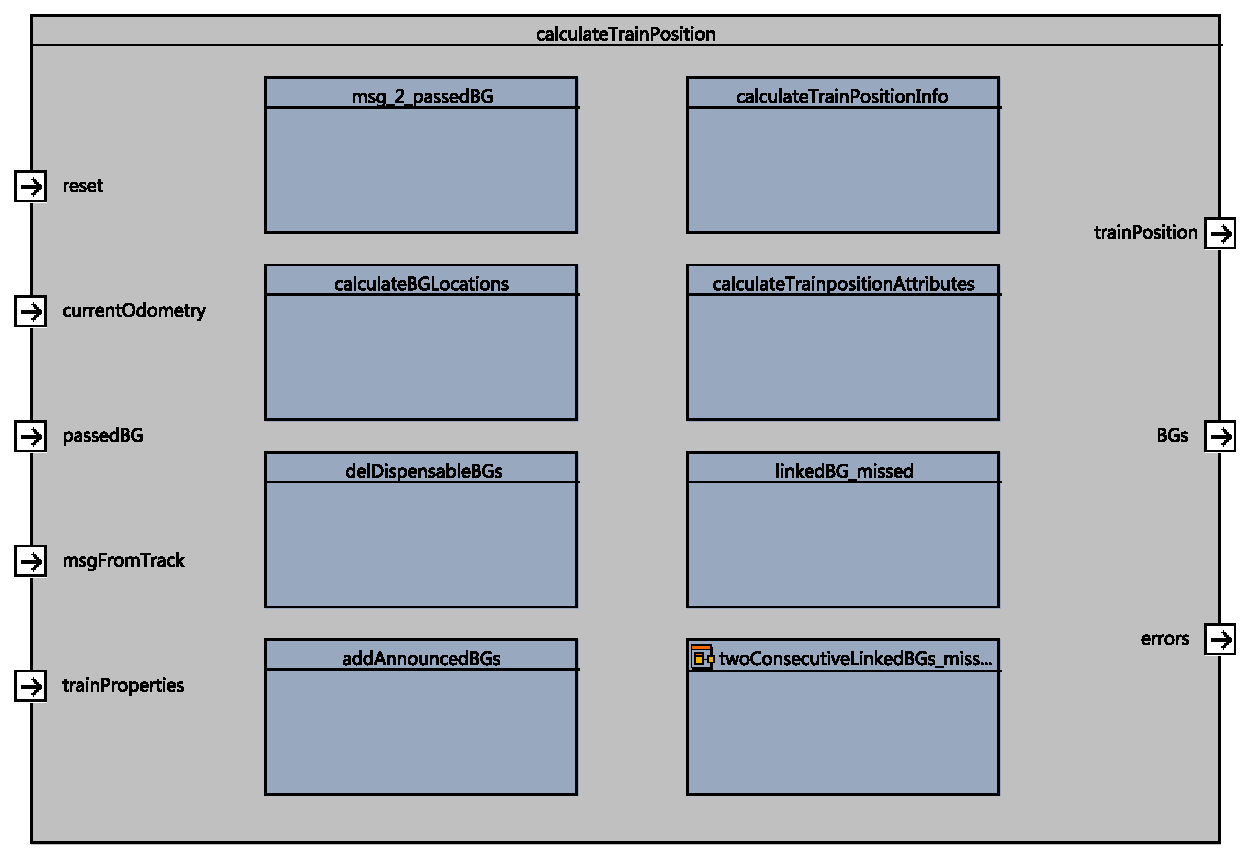
\includegraphics[width=\textwidth]{./images/F2_6_calculateTrainPosition.pdf}
	\caption{calculateTrainPosition component SysML diagram.}
	\label{f:calculateTrainPosition_interface}
\end{figure}


\subsubsection{Inputs}\label{s:calculateTrainPosition_inputs}

\paragraph{currentOdometry}

\begin{longtable}{p{.25\textwidth}p{.7\textwidth}}
\toprule
Input name				& currentOdometry \\
\midrule
Description				& currentOdometry is the actual odometry information as known by the whole EVC model and provided by the models external interface. \\
\midrule
Source					& F2 input API\_Odometry \\ 
\midrule
Type					& Obu\_BasicTypes\_Pkg::odometry\_T \\  
\midrule
Valid range of values	& Obu\_BasicTypes\_Pkg::odometry\_T is a complex data type. Values are given for each element. Format is: Type Name: range / list of values.
\begin{itemize}
\item bool valid: [true | false]. Must be permanently set to "true".
\item timestamp: (0 - 2147483647). Current time in ms, must be monotonically increasing.
\item odo: Obu\_BasicTypes\_Pkg::OdometryLocations\_T: current odometry log values with uncertainties; must behave according to {\footnotesize\url{https://github.com/openETCS/SRS-Analysis/blob/master/System%20Analysis/WorkingRepository/Group4/SUBSET_26_3-6/DetermineTrainLocationProcedures.pdf}} [[ 3.1 ]]. Members of OdometryLocations\_T are: 
  \begin{itemize}
  \item o\_nominal: L\_internal\_Type: nominal value in cm.
  \item o\_min:     L\_internal\_Type: \newline min. distance = o\_min2 - o\_min1
  \item o\_max:     L\_internal\_Type: \newline max distance = o\_max2 - o\_max1
  \end{itemize}
\item speed: Obu\_BasicTypes\_Pkg::OdometrySpeeds\_T: not used by calculateTrainPosition
\item acceleration: Obu\_BasicTypes\_Pkg::A\_internal\_Type: not used by calculateTrainPosition
\item motionState: [noMotion | Motion]
\item motionDirection: Obu\_BasicTypes\_Pkg::odoMotionDirection\_T \newline [ unknownDirection | cabAFirst | cabBFirst ]
\end{itemize}
\emph{calculateTrainPosition requires consistent value sets of currentOdometry. calculateTrainPosition itself does not check.  }\\
\midrule
Behaviour when value is at boundary	& n/a \\
\midrule
Behaviour for values out of valid range	& Enumerated values out of range prohibit code generation. In all other cases, calculateTrainPosition does not have the knowledge for out-of-range checks. \\
\midrule
Behaviour when value is erroneous, absent or unwanted (i.e. spurious) & Leads to misbehaviour. \\
\bottomrule
\end{longtable}



\paragraph{msgFromTrack}

\begin{longtable}{p{.25\textwidth}p{.7\textwidth}}
\toprule
Input name				& msgFromTrack \\
\midrule
Description				& With msgFromTrack calculateTrainPosition receives datagrams from balise groups and RBC. \\
\midrule
Source					& F2.1 Manage\_TrackSideInformation\_Integration \\ 
\midrule
Type					& Common\_Types\_Pkg::ReceivedMessage\_T \\  
\midrule
Valid range of values	& Common\_Types\_Pkg::ReceivedMessage\_T is a complex data type. Values are given for each element. Format is: Type Name: range / list of values.
\begin{itemize}
	\item bool valid: [true | false]. "true" flags a datagram as received and to be evaluated by calculateTrainPosition. Must be set for exactly 1 clock for each received datagram and stay unset otherwise.

	\item source: Common\_Types\_Pkg::MsgSource\_T: Designates the source of the datagram: \newline ( msrc\_undefined | msrc\_Euroradio | msrc\_Eurobalise | msrc\_RadioInfillUnit | msrc\_OBU ) 

	\item radioMetaData: Common\_Types\_Pkg::radioMetaData\_T: not used by calculateTrainPosition.

	\item BG\_Common\_Header: BG\_Types\_Pkg::BG\_Header\_T: Header information received from balise groups, refer to Manage\_TrackSideInformation\_Integration\_Pkg::\newline Manage\_TrackSideInformation\_Integration

	\item Radio\_Common\_Header: Radio\_Types\_Pkg::Radio\_TrackTrain\_Header\_T: Header information received from RBC via radio, refer to Manage\_TrackSideInformation\_Integration\_Pkg::\newline Manage\_TrackSideInformation\_Integration

	\item packets: Common\_Types\_Types\_Pkg::CompressedPackets\_T: datagram packets, refer to Manage\_TrackSideInformation\_Integration\_Pkg::\newline Manage\_TrackSideInformation\_Integration. calculatesTrainPosition extracts packet 5 (linking information), if available.

	\item sendingRBC: Common\_Types\_Types\_Pkg::RBC\_Id\_T: designates the origin RBC and the mobile modem channel used onboard, if received via radio. Refer to Manage\_TrackSideInformation\_Integration\_Pkg::\newline Manage\_TrackSideInformation\_Integration for more detailed information.
\end{itemize}  
\emph{calculateTrainPosition expects the received information to be consistent and validated before applied to. It does not check, if the information is appropriate due to current EVC mode, level, train or balise orientation. Received balise group or linking information already known by calculateTrainPosition overrides former data. All messages must be applied in the correct chronological order} \\
\midrule
Behaviour when value is at boundary	& n/a \\
\midrule
Behaviour for values out of valid range	& Enumerated values out of range prohibit code generation. In all other cases, calculateTrainPosition does not have the knowledge for out-of-range checks. \\
\midrule
Behaviour when value is erroneous, absent or unwanted (i.e. spurious) & Causes misbehaviour.
\\
\bottomrule
\end{longtable}


\paragraph{trainProperties}

\begin{longtable}{p{.25\textwidth}p{.7\textwidth}}
\toprule
Input name				& trainProperties \\
\midrule
Description				& Supplies calculateTrainPosition with train specific properties required for position calculation.   \\
\midrule
Source					& F2.3 trainData\newline
F2.10 manageDMI\_input \\ 
\midrule
Type					& TrainPosition\_Types\_Pck::trainProperties\_T \\  
\midrule
Valid range of values	& TrainPosition\_Types\_Pck::trainProperties\_T is a complex data type. Values are given for each element. Format is: Type Name: range / list of values.
\begin{itemize}
\item nid\_engine:: NID\_ENGINE as defined by subset 026-7. 
\item nid\_operational: NID\_OPERATIONAL as defined by subset 026-7. 
\item l\_train: L\_TRAIN as defined by subset 026-7. 
\item d\_baliseAntenna\_2\_frontend: Obu\_BasicTypes\_Pkg::LocWithInAcc\_T:  Distance from the trains balise antenna to the trains front end, in cm with uncertainties. 
\item d\_frontend\_2\_rearend: Obu\_BasicTypes\_Pkg::LocWithInAcc\_T:  Distance from the trains Distance from the trains front end to rear end, in cm with uncertainties. 
\item locationAccuracy\_DefaultValue: Obu\_BasicTypes\_Pkg::LocWithInAcc\_T:  Default location accuracy of balise groups (subset 026, 3.6.4.3.2), in cm with uncertainties. 
\item centerDetectionAcc\_DefaultValue: Obu\_BasicTypes\_Pkg::LocWithInAcc\_T:  Default  accuracy of balise groups detection of the BTM, in cm with uncertainties. Will be applied, if centerDetectionInaccuracy from BTM is not available, especially for announced and not yet passed BGs. 
\end{itemize} 
\emph{calculateTrainPosition expects this information to be consistent and validated before applied to.}\\
\midrule
Behaviour when value is at boundary	& n/a \\
\midrule
Behaviour for values out of valid range	& Enumerated values out of range prohibit code generation. In all other cases, calculateTrainPosition does not have the knowledge for out-of-range checks. \\
\midrule
Behaviour when value is erroneous, absent or unwanted (i.e. spurious) & Causes misbehaviour.
\\
\bottomrule
\end{longtable}



\paragraph{passedBG}

\begin{longtable}{p{.25\textwidth}p{.7\textwidth}}
\toprule
Input name				& passedBG \\
\midrule
Description				& Deprecated alternative input to msgFromTrack. Must not be used any more and is subject to be removed in subsequent releases.  \\
\bottomrule
\end{longtable}


\paragraph{reset}

\begin{longtable}{p{.25\textwidth}p{.7\textwidth}}
\toprule
Input name				& reset \\
\midrule
Description				& Resets and keeps calculateTrainPosition at its initial state and deletes all internally stored data.  \\
\midrule
Source					& F2 input EVC\_reset \\ 
\midrule
Type					& bool \\  
\midrule
Valid range of values	& [ false | true ] \\
\midrule
Behaviour when value is at boundary	& n/a \\
\midrule
Behaviour for values out of valid range	& Enumerated values out of range prohibit code generation. \\
\midrule
Behaviour when value is erroneous, absent or unwanted (i.e. spurious) & Causes misbehaviour.
\\
\bottomrule
\end{longtable}


\subsubsection{Outputs}\label{s:calculateTrainPosition_outputs}

\paragraph{trainPosition}

\begin{longtable}{p{.25\textwidth}p{.7\textwidth}}
\toprule
Output name				& trainPosition \\
\midrule
Description				& Provides the current train position and LRBG with its attributes. All distance and location computations of the OBU must be based on this information.   \\
\midrule
Destination				& F2.1 Manage\_TracksideInformation\_Integration\newline
F2.2 Manage\_ETCS\_Procedures\newline
F2.4 TrackAtlas\newline
F2.5 ManageLevelAndMode\newline
F2.7 PeedSupervision\_Integration\newline
F2.8 ProvidePositionReport\newline
F2.9 MORC\_HO\newline
F2.11 manageDMI\_Output
\\ 
\midrule
Type					& TrainPosition\_Types\_Pck::trainPosition\_T \\  
\midrule
Valid range of values	& TrainPosition\_Types\_Pck::trainPosition\_T is a complex data type. Values are given for each element. Format is: Type Name: range / list of values.
\begin{itemize}
\item valid: bool: [true | false]. Always true, except for exceptional circumstances.
\item timestamp: Obu\_BasicTypes\_Pkg::T\_internal\_Type: latest time in ms. 
\item trainPositionIsUnknown: bool: true, if the train position is evaluated as "unknonwn" (refer to subset-026, 3.6.3.1.3.1). 
\item noCoordinateSystemHasBeenAssigned: bool: refer to subset 026, 3.4.2, 3.6.3.1.4.
\item trainPosition: Obu\_BasicTypes\_Pkg::LocWithInAcc\_T: The calculated train position with uncertainties
\item estimatedFrontEndPosition: Obu\_BasicTypes\_Pkg::Location\_T: Train front end position in cm.
\item minSafeFrontEndPosition: Obu\_BasicTypes\_Pkg::Location\_T: Train front end position in cm.
\item maxSafeFrontEndPostion: Obu\_BasicTypes\_Pkg::Location\_T: Train front end position in cm.
\item LRBG: TrainPosition\_Types\_Pck::positionedBG\_T: the current LRBG. 
\item prvLRBG: TrainPosition\_Types\_Pck::positionedBG\_T: the balise group passed previously to LRBG. For type definition, see below.
\item nominalOrReverseToLRBG: Q\_DLRBG: Orientation of the train in relation to the direction of the LRBG, see subset 026-7.
\item trainOrientationToLRBG: Q\_DIRLRBG: Orientation of the train in relation to the direction of the LRBG, see subset 026-7.
\item trainRunningDirectionToLRBG: Q\_DIRTRAIN: Direction of train movement in relation to the LRBG orientation, see subset 026-7.
\item linkingIsUsedOnboard: bool: Designates, if at least one announced linked BG is ahead.
\end{itemize} 
\\
\midrule
Behaviour when value is at boundary	& n/a \\
\midrule
Behaviour for values out of valid range	& n/a \\
\midrule
Behaviour when value is errorneous, absent or unwanted & n/a \\
\bottomrule
\end{longtable}


\paragraph{BGs}

\begin{longtable}{p{.25\textwidth}p{.7\textwidth}}
\toprule
Output name				& BGs \\
\midrule
Description				& A list of all linked and unlinked balise groups - known to calculateTrainPosition - in the order they are arranged on the track.   \\
\midrule
Destination				& F2.1 Manage\_TracksideInformation\_Integration\newline
F2.8 ProvidePositionReport\newline
F2.9 MoRC\_HO \\ 
\midrule
Type					& array of TrainPosition\_Types\_Pck::positionedBG\_T \\  
\midrule
Valid range of values	& TrainPosition\_Types\_Pck::positionedBG\_T is a complex data type. Values are given for each array element. Format is: Type Name: range / list of values.
\begin{itemize}
	\item valid: bool: [true | false]. "true" for every existing balise group.
	\item nid\_c: NID\_C: refer to subset 026-7. 
	\item nid\_bg: NID\_BG: refer to subset 026-7. 
	\item q\_link: Q\_LINK: refer to subset 026-7. 
	\item location: Obu\_BasicTypes\_Pkg::LocWithInAcc\_T: The best known location (with inaccuracies) calculated from linking and from passing information.
	\item seqNoOnTrack: int: Sequence number, specifies the order of the BG passed or expected to be passed.
	\item infoFromLinking: TrainPosition\_Types\_Pck::infoFromLinking\_T: Describes a linked BG as announced from the linking BG. Mainly, this information is taken from the linking packet.
	\item infoFromPassing: BG\_Types\_Pkg::passedBG\_T: If the balise group has been passed already, this is the relevant information received from the BG.
\end{itemize} 
\\
\midrule
Behaviour when value is at boundary		& n/a \\
\midrule
Behaviour for values out of valid range	& n/a \\
\midrule
Behaviour when value is errorneous, absent or unwanted & n/a \\
\bottomrule
\end{longtable}


\paragraph{errors}

\begin{longtable}{p{.25\textwidth}p{.7\textwidth}}
\toprule
Output name				& errors \\
\midrule
Description				& Provides a collection of error flags, raised by calculateTrainPosition.   \\
\midrule
Destination				& F2.5 ManageLevelAndMode\newline
F2.8 ProvidePositionReport \\ 
\midrule
Type					& TrainPosition\_Types\_Pck::positionErrors\_T \\  
\midrule
Valid range of values	& TrainPosition\_Types\_Pck::positionErrors\_T is a complex data type. Values are given for each array element. Format is: Type Name: range / list of values.
\begin{itemize}
\item outOfMemSpace: bool: Memory overrun: a passed or announced BG could not be stored.
\item passedBG\_foundNotWhereExpected: bool: The currently passed linked BG location does not match its expectation window.
\item positionCalculation\_inconsistent: A consistency problem arose during position calculation.
\item linkedBGMissed: bool: The expectation window for an announced BG was passed without detecting the BG.
\item BGpassedInUnexpectedDirection: bool: The BG was passed in a different orientation than announced via linking.
\item BG\_LinkingConsistencyError: bool: Linking consistency error (ref. subset 026, 3.16.2.3).
\item twoConsecutiveLinkedBGs\_missed: bool: 2 consecutive linked balise groups announced by linking are not detected and the end of the expectation window of the second balise group has been passed (subset 026, 3.16.2.7.1).
\item doubleRepositioningError: bool: Double repositioning error (3.16.2.7.2).
\item bg: TrainPosition\_Types\_Pck::positionedBG\_T: The corresponding balise group in the case of an error.
\end{itemize}  \\
\midrule
Behaviour when value is at boundary		& n/a \\
\midrule
Behaviour for values out of valid range	& n/a \\
\midrule
Behaviour when value is errorneous, absent or unwanted & n/a \\
\bottomrule
\end{longtable}


\subsection{Subcomponents}\label{s:calculateTrainPosition_subcomponents}

\subsubsection{msg\_2\_passedBG}
%set the master document for easy compilation
%!TEX root = ../D3_5_3.tex

\paragraph{Component Requirements}

\begin{longtable}{p{.25\textwidth}p{.7\textwidth}}
\toprule
Component name			& msg\_2\_passedBG \\
\midrule
Link to SCADE model		& {\footnotesize \url{http://???}} \\
\midrule
SCADE designer			& Uwe Steinke, Siemens AG \\
\midrule
Description				& [Brief description of the components functionality] \\
\midrule
Input documents	& 
Subset-026, Chapter ?.?\newline
Subset-026, Chapter ?.?\newline
Subset-026, Chapter ?.?.?\\
\midrule
Safety integrity level	& 4 \\
\midrule
Time constraints		& [If applicable description of time constraints, otherwise n/a] \\
\midrule
API requirements 		& [If applicable description of API requirements, otherwise n/a] \\
\bottomrule
\end{longtable}


\paragraph{Interface}

For an overview of the interface of this internal component we refer to the SCADE model (cf.~link above) respectively the SCADE generated documentation.

\subsubsection{calculateBGLocations}
%set the master document for easy compilation
%!TEX root = ../D3_5_3.tex

\paragraph{Component Requirements}

\begin{longtable}{p{.25\textwidth}p{.7\textwidth}}
\toprule
Component name			& calculateBGLocations \\
\midrule
Link to SCADE model		& {\footnotesize \url{http://???}} \\
\midrule
SCADE designer			& Uwe Steinke, Siemens AG \\
\midrule
Description				& [Brief description of the components functionality] \\
\midrule
Input documents	& 
Subset-026, Chapter ?.?\newline
Subset-026, Chapter ?.?\newline
Subset-026, Chapter ?.?.?\\
\midrule
Safety integrity level		& 4 \\
\midrule
Time constraints		& [If applicable description of time constraints, otherwise n/a] \\
\midrule
API requirements 		& [If applicable description of API requirements, otherwise n/a] \\
\bottomrule
\end{longtable}


\paragraph{Interface}

For an overview of the interface of this internal component we refer to the SCADE model (cf.~link above) respectively the SCADE generated documentation.

\subsubsection{delDispensableBGs}
%set the master document for easy compilation
%!TEX root = ../D3_5_3.tex

\paragraph{Component Requirements}

\begin{longtable}{p{.25\textwidth}p{.7\textwidth}}
\toprule
Component name			& delDispensableBGs \\
\midrule
Link to SCADE model		& {\footnotesize \url{http://???}} \\
\midrule
SCADE designer			& [Name, affiliation] \\
\midrule
Description				& [Brief description of the components functionality] \\
\midrule
Input documents	& 
Subset-026, Chapter ?.?\newline
Subset-026, Chapter ?.?\newline
Subset-026, Chapter ?.?.?\\
\midrule
Safety integrity level		& 4 \\
\midrule
Time constraints		& [If applicable description of time constraints, otherwise n/a] \\
\midrule
API requirements 		& [If applicable description of API requirements, otherwise n/a] \\
\bottomrule
\end{longtable}


\paragraph{Interface}

For an overview of the interface of this internal component we refer to the SCADE model (c.f.~link above) respectively the SCADE generated documentation.

\subsubsection{addAnnouncedBGs}
%set the master document for easy compilation
%!TEX root = ../D3_5_3.tex

\paragraph{Component Requirements}

\begin{longtable}{p{.25\textwidth}p{.7\textwidth}}
\toprule
Component name			& addAnnounceBGs \\
\midrule
Link to SCADE model		& {\footnotesize \url{http://???}} \\
\midrule
SCADE designer			& [Name, affiliation] \\
\midrule
Description				& [Brief description of the components functionality] \\
\midrule
Input documents	& 
Subset-026, Chapter ?.?\newline
Subset-026, Chapter ?.?\newline
Subset-026, Chapter ?.?.?\\
\midrule
Safety integrity level		& 4 \\
\midrule
Time constraints		& [If applicable description of time constraints, otherwise n/a] \\
\midrule
API requirements 		& [If applicable description of API requirements, otherwise n/a] \\
\bottomrule
\end{longtable}


\paragraph{Interface}

For an overview of the interface of this internal component we refer to the SCADE model (c.f.~link above) respectively the SCADE generated documentation.

\subsubsection{calculateTrainpositionInfo}
%set the master document for easy compilation
%!TEX root = ../D3_5_3.tex

\paragraph{Component Requirements}

\begin{longtable}{p{.25\textwidth}p{.7\textwidth}}
\toprule
Component name			& calculateTrainpositionInfo \\
\midrule
Link to SCADE model		& {\footnotesize \url{http://???}} \\
\midrule
SCADE designer			& [Name, affiliation] \\
\midrule
Description				& [Brief description of the components functionality] \\
\midrule
Input documents	& 
Subset-026, Chapter ?.?\newline
Subset-026, Chapter ?.?\newline
Subset-026, Chapter ?.?.?\\
\midrule
Safety integrity level		& 4 \\
\midrule
Time constraints		& [If applicable description of time constraints, otherwise n/a] \\
\midrule
API requirements 		& [If applicable description of API requirements, otherwise n/a] \\
\bottomrule
\end{longtable}


\paragraph{Interface}

For an overview of the interface of this internal component we refer to the SCADE model (c.f.~link above) respectively the SCADE generated documentation.

\subsubsection{calculateTrainPositionAttributes}
%set the master document for easy compilation
%!TEX root = ../D3_5_3.tex

\paragraph{Component Requirements}

\begin{longtable}{p{.25\textwidth}p{.7\textwidth}}
\toprule
Component name			& calculateTrainPositionAttributes \\
\midrule
Link to SCADE model		& {\footnotesize \url{http://???}} \\
\midrule
SCADE designer			& Uwe Steinke, Siemens AG \\
\midrule
Description				& [Brief description of the components functionality] \\
\midrule
Input documents	& 
Subset-026, Chapter ?.?\newline
Subset-026, Chapter ?.?\newline
Subset-026, Chapter ?.?.?\\
\midrule
Safety integrity level		& 4 \\
\midrule
Time constraints		& [If applicable description of time constraints, otherwise n/a] \\
\midrule
API requirements 		& [If applicable description of API requirements, otherwise n/a] \\
\bottomrule
\end{longtable}


\paragraph{Interface}

For an overview of the interface of this internal component we refer to the SCADE model (cf.~link above) respectively the SCADE generated documentation.

\subsubsection{linkedBG\_missed}
%set the master document for easy compilation
%!TEX root = ../D3_5_3.tex

\paragraph{Component Requirements}

\begin{longtable}{p{.25\textwidth}p{.7\textwidth}}
\toprule
Component name			& linkedBG\_missed \\
\midrule
Link to SCADE model		& {\footnotesize \url{http://???}} \\
\midrule
SCADE designer			& Uwe Steinke, Siemens AG \\
\midrule
Description				& [Brief description of the components functionality] \\
\midrule
Input documents	& 
Subset-026, Chapter ?.?\newline
Subset-026, Chapter ?.?\newline
Subset-026, Chapter ?.?.?\\
\midrule
Safety integrity level		& 4 \\
\midrule
Time constraints		& [If applicable description of time constraints, otherwise n/a] \\
\midrule
API requirements 		& [If applicable description of API requirements, otherwise n/a] \\
\bottomrule
\end{longtable}


\paragraph{Interface}

For an overview of the interface of this internal component we refer to the SCADE model (cf.~link above) respectively the SCADE generated documentation.

\subsubsection{twoconsecutiveLinkedBGs\_missed}
%set the master document for easy compilation
%!TEX root = ../D3_5_3.tex

\paragraph{Component Requirements}

\begin{longtable}{p{.25\textwidth}p{.7\textwidth}}
\toprule
Component name			& twoconsecutiveLinkedBGs\_missed \\
\midrule
Link to SCADE model		& {\footnotesize \url{http://???}} \\
\midrule
SCADE designer			& Uwe Steinke, Siemens AG \\
\midrule
Description				& [Brief description of the components functionality] \\
\midrule
Input documents	& 
Subset-026, Chapter ?.?\newline
Subset-026, Chapter ?.?\newline
Subset-026, Chapter ?.?.?\\
\midrule
Safety integrity level		& 4 \\
\midrule
Time constraints		& [If applicable description of time constraints, otherwise n/a] \\
\midrule
API requirements 		& [If applicable description of API requirements, otherwise n/a] \\
\bottomrule
\end{longtable}


\paragraph{Interface}

For an overview of the interface of this internal component we refer to the SCADE model (cf.~link above) respectively the SCADE generated documentation.






